%%%%%%%%%%%%%%%%%%%%%%%%%%%%%%%%%%%%%%%%%%%%%%%%%
%%%%      SECTION 2 — BioGen NL Agent        %%%%
%%%%   §2a  Data, Indexing & Search (Ph.1)   %%%%
%%%%%%%%%%%%%%%%%%%%%%%%%%%%%%%%%%%%%%%%%%%%%%%%%

\section{BioGen NL Agent}
\label{sec:biogen}

\subsection{Data Parsing, Indexing and Search (Phase~1)}
\label{sec:phase1}

% ── 2a.1  DATA ────────────────────────────────────────────────────────────────
\subsubsection{Data}

The collection comprises 4{,}194 PubMed abstracts with a mean length of
150~words (median 142, range 12--964).
We use the 65 TREC BioGen 2024 topics (IDs~116--180) distributed in
\texttt{BioGen2024topics.json}.  Each topic contains three fields:
a short keyword \texttt{topic} (2--6 words), a natural-language clinical
\texttt{question} (10--20 words), and a longer \texttt{narrative} providing
retrieval context (30--70 words).

Relevance judgements are derived from
\texttt{biogen\_2024\_\allowbreak submissions\allowbreak .json},
which contains automated BioGen~2024 system submissions annotated with
sentence-level citation assessments (the \texttt{evidence\_relation} field).
We construct two relevance scales --- \emph{binary}
(supporting\,=\,1, else\,=\,0) and \emph{graded}
(supporting\,=\,5, neutral\,=\,2, else\,=\,0) --- to support
different evaluation metrics.  Full construction details and the
train/test split protocol appear in §\ref{sec:eval_setup}.

% ── 2a.2  INDEXING AND RETRIEVAL METHODS ──────────────────────────────────────
\subsubsection{Indexing and Retrieval Methods}

All documents are stored in a single OpenSearch index
(\texttt{usernlp03}) on the shared course instance~\cite{opensearch},
with one field per parameter configuration so that BM25 and
language-model scores are pre-computed at index time and available
instantly at query time.
A baseline pass creates the default fields and a tuning pass extends the
index with the full parameter grid ($\approx$45~fields total), managed
idempotently by \texttt{index\_builder.py}.
We use the \texttt{standard} analyser (tokenise + lowercase) rather than
\texttt{english}, because Porter stemming mangles biomedical terms
(e.g.\ \emph{hepatitis} $\to$ \emph{hepat}).
For KNN fields, vectors are L2-normalised before indexing so that
\texttt{innerproduct} is equivalent to cosine similarity
(\texttt{ef\_construction}\,=\,256, $M$\,=\,48,
\texttt{ef\_search}\,=\,100).

\paragraph{Sparse retrievers:}
We implement three lexical strategies sharing a uniform interface
(\texttt{BaseRetriever.search(query, size=100)}).
\textbf{BM25}~\cite{robertson1994bm25} is a probabilistic term-weighting
model where $k_1$ controls term-frequency saturation and $b$ governs
length normalisation (defaults: $k_1$\,=\,1.2, $b$\,=\,0.75; tuned in
§\ref{sec:eval_results}).
\textbf{LM~Jelinek-Mercer} smooths the document language model via linear
interpolation with the collection model ($\lambda$\,=\,0.7).
\textbf{LM~Dirichlet}~\cite{lm_retrieval} applies Dirichlet-prior
smoothing ($\mu$\,=\,2{,}000).

\paragraph{Dense retriever:}
\textbf{KNN} performs HNSW approximate nearest-neighbour search on
768-dimensional embeddings.
Our baseline encoder is
\texttt{msmarco-distilbert-base-v2}~\cite{reimers2019sbert};
we also evaluate
\texttt{multi-qa-mpnet}~\cite{reimers2019sbert},
\texttt{allenai/specter2}, and
\texttt{ncbi/MedCPT}~\cite{medcpt2023} --- an asymmetric dual-encoder
trained on 23M PubMed click-through pairs that is an exact domain match
for our task.
Before comparing encoder families we evaluate three pooling modes
(\emph{mean}, \emph{mean-no-special}, \emph{CLS}) for every encoder via
brute-force exact cosine (no HNSW approximation); Figure~\ref{fig:pooling}
shows the results, with CLS winning for MedCPT and SPECTER-2 while
mean-no-special is preferable for msmarco and multi-qa.
Each encoder's best pooling mode is locked for all subsequent experiments;
full comparison results appear in §\ref{sec:eval_results}.

\begin{figure}[htbp]
  \centering
  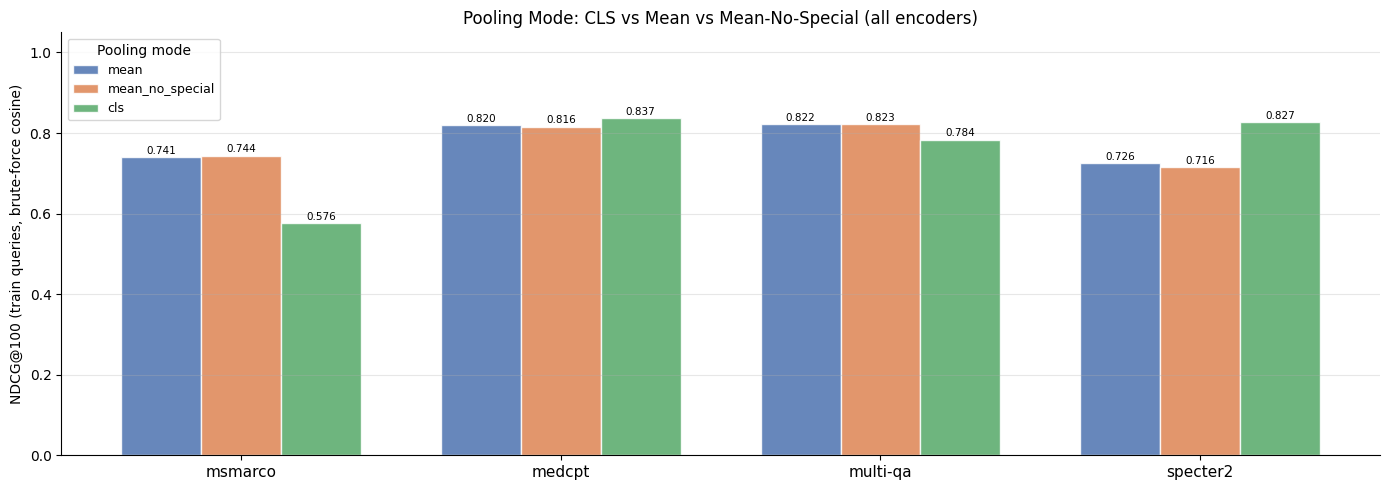
\includegraphics[width=\linewidth]{images/pooling_mode_sweep.png}
  \caption{Pooling-mode comparison --- NDCG@100 for each encoder $\times$
           pooling mode (brute-force exact cosine on 32 train topics).
           MedCPT + CLS yields the highest single score (0.8374).}
  \label{fig:pooling}
\end{figure}

\paragraph{Hybrid fusion:}
\textbf{Reciprocal Rank Fusion (RRF)}~\cite{rrf2009} merges two ranked lists
in a score-agnostic manner:
$\text{RRF}(d)=\sum_r \frac{1}{k + \text{rank}_r(d)}$, with $k$\,=\,60.
We fuse BM25 with KNN\,(MedCPT), chosen because lexical and semantic
signals are largely complementary.
